\documentclass[a4paper,10pt]{article}

\usepackage[utf8]{inputenc}
\usepackage[english]{babel}
%\usepackage[T1]{fontenc}
\usepackage{graphicx}
\usepackage{wrapfig}
\usepackage{amsmath, amssymb}
%\usepackage{listings}
\usepackage{float}
\begin{document}

\author{Valentin Rosenberg, Zacharias Dyna Knudsen}
\date{\today}

\tableofcontents
\newpage

\section{Introduction}
The data combines socio-economic data from the 1990 US Census, law enforcement data from the 1990 US LEMAS (Law Enforcement Management And Administrative Statistics) survey, and crime data from the 1995 FBI UCR (Uniform Crime Reporting). The main problem of interest intended with the data is the prediction of crimes.
The data was obtained from http://archive.ics.uci.edu/ml/\newline
datasets/Communities+and+Crime+Unnormalized. We also looked at a normalized version of this dataset from http://archive.ics.uci.edu/ml/datasets/Co-\newline
mmunities+and+Crime that has been normalized with a unsupervised, equal-interval binning method. The data has previously been used to predict violent crimes per population. 
The primary machine learning task is regression, as the data is a collection of attributes that are thought to be related to the number of crimes. We would like to predict the autotheft attribute with a regression model using the data as training set. As a classification problem we could predict whether new data objects belong to a rich/poor community or a colored/white community. We would also like to find groups of communities that are similar to eachother based on socio-economic attributes. We could also detect communities with deviating from the normal of communities with anomaly detection. 
\section{Detailed description of the data} 
There was apparently a limitation to this dataset, which was that the LEMAS survey was of the police departments with at least 100 officers, plus a random sample of smaller departments, so many communities are missing values in police related attributes, as we can also see in the summary statistic in the appendix. There was also some controversy in some states concerning the counting of rapes. These resulted in missing values for rape, which resulted in incorrect values for per capita violent crime. These cities are not included in the dataset. Many of these omitted communities were from the midwestern USA. Our data consists of 147 attributes, most of which are discrete or continous ratios. For example there is a population attribute for each community, and a householdsize attribute which is the mean number of people per household in the community. There are also nominal attributes, one with the names of the community and the state's name. LemanGangUnitDeploy is a nominal discrete attribute where 0 means no gangunit deployed and 1 means there is a gangunit, and 0.5 means a part-time gang unit is deployed. 
Many of the attributes have missing values which are represented by a questionmark in the dataset. These we will try to deal with in various ways. We will try to estimate the mean, delete the data objects and delete the attributes with the missing values.
The statistical summary also shows that it seems pctblack and pctwhite have high correlation with crimes per population as well as the attributes concerning families with two parents.

\section{Visualisation}
Based on a principal component analysis of the data (excluding the first columns including only identifier information like state names) there appear to be some potential problems with outliers. In all PCA illustrations, the colors represent amount of auto theft.

\begin{figure}[H]
\centering
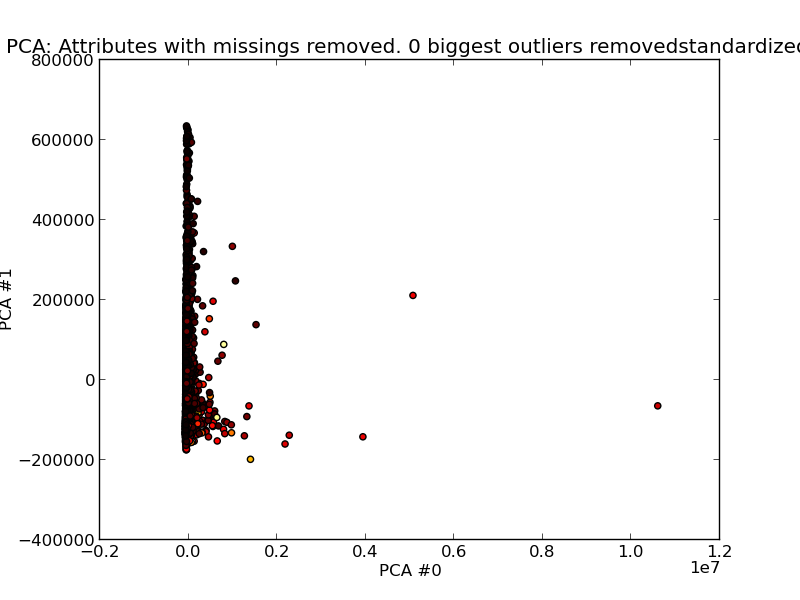
\includegraphics[width=0.9\textwidth]{pca/attr-with-missings-removed_0-biggest-outliers-removed_standrd_}
\label{fig:prenorm_attrrem_0out}
\caption{PCA, where attributes with missing values have been removed removed.}
\end{figure}

We are not yet sure how best to deal with these, but in order to explore our data we also performed principal componenet analysis on our data set with some of the biggest outliers removed.

\begin{figure}[H]
\centering
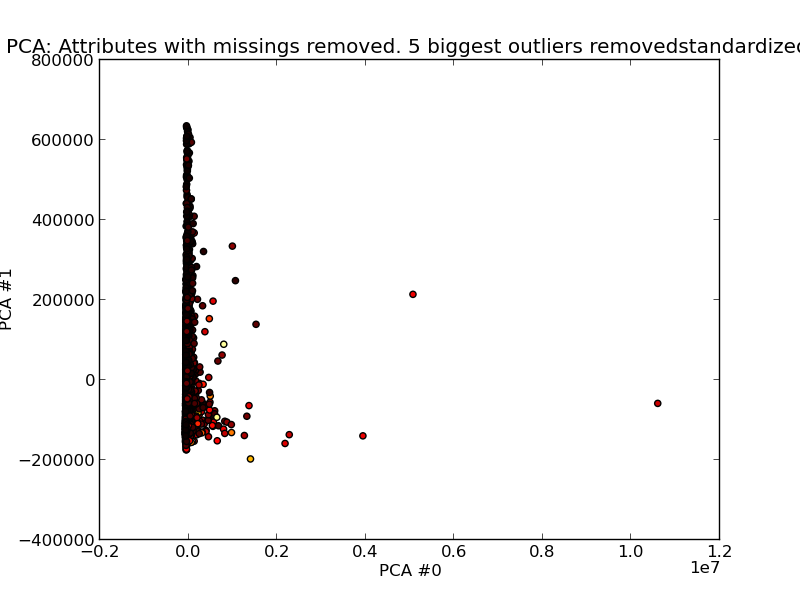
\includegraphics[width=0.9\textwidth]{pca/attr-with-missings-removed_5-biggest-outliers-removed_standrd_}
\label{fig:prenorm_attrrem_0out}
\caption{PCA, where attributes with missing values have been removed removed. Also the 5 biggest outliers from before have been removed prior to PCA.}
\end{figure}

The above pictures illustrate our results, when we dealt with missing values by removing the corresponding attribute completely. We also performed PCA after removing data objects with missing values instead, see below


\begin{figure}[H]
\centering
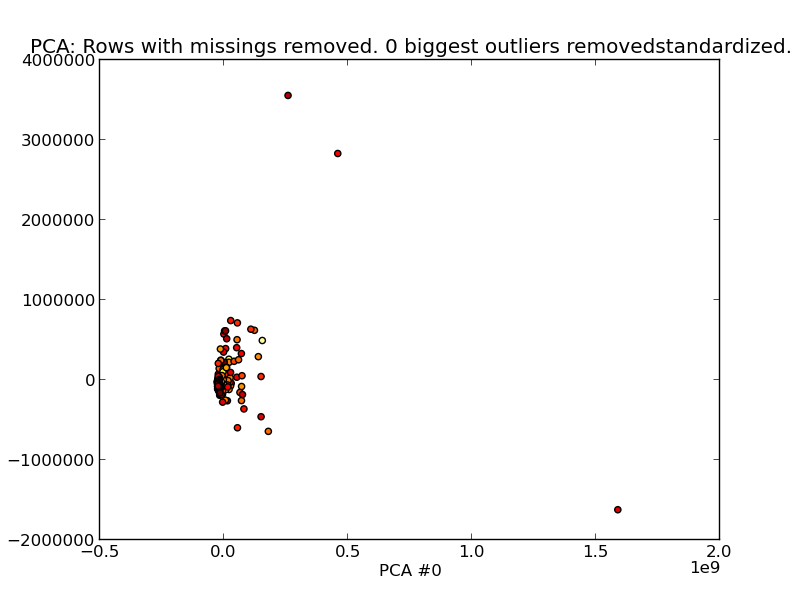
\includegraphics[width=0.9\textwidth]{pca/rows-with-missings-removed_0-biggest-outliers-removed_standrd_}
\label{fig:prenorm_attrrem_0out}
\caption{PCA, where data objects with missing values have been removed removed.}
\end{figure}
\begin{figure}[H]
\centering
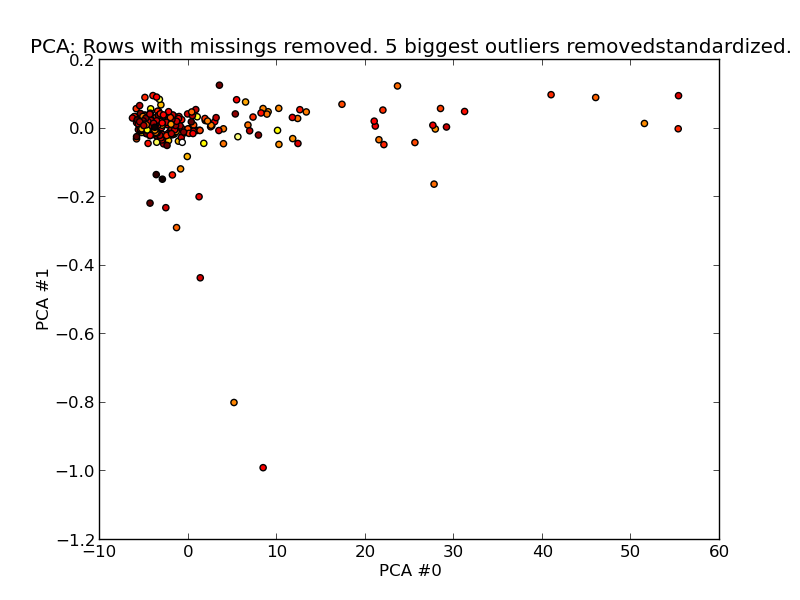
\includegraphics[width=0.9\textwidth]{pca/rows-with-missings-removed_5-biggest-outliers-removed_standrd_}
\label{fig:prenorm_attrrem_0out}
\caption{PCA, where data objects with missing values have been removed removed. Also the 5 biggest outliers from before have been removed prior to PCA.}
\end{figure}

We also did PCA where we simply put the means along attributes instead of missing values, producing the following principal components.

\begin{figure}[H]
\centering
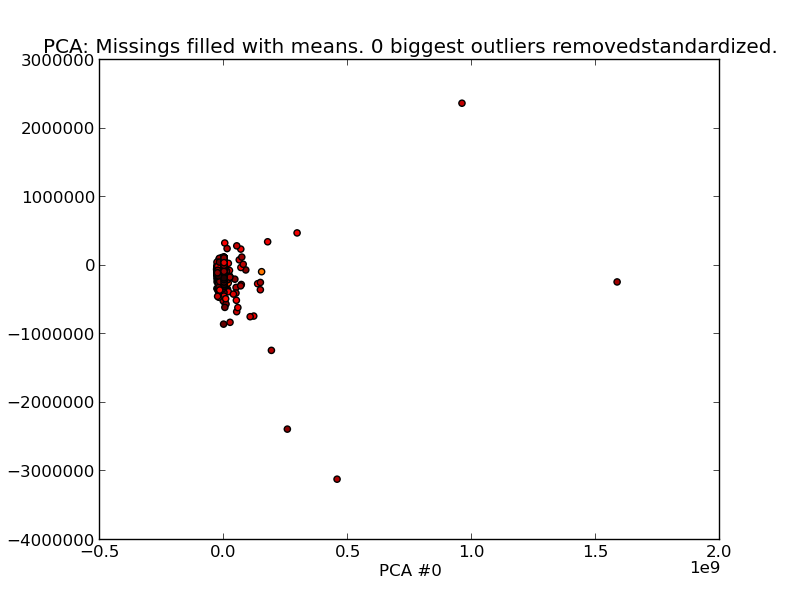
\includegraphics[width=0.9\textwidth]{pca/missings-filled-w-means_0-biggest-outliers-removed_standrd_}
\label{fig:prenorm_attrrem_0out}
\caption{PCA, where missing values have been replaced with means.}
\end{figure}
\begin{figure}[H]
\centering
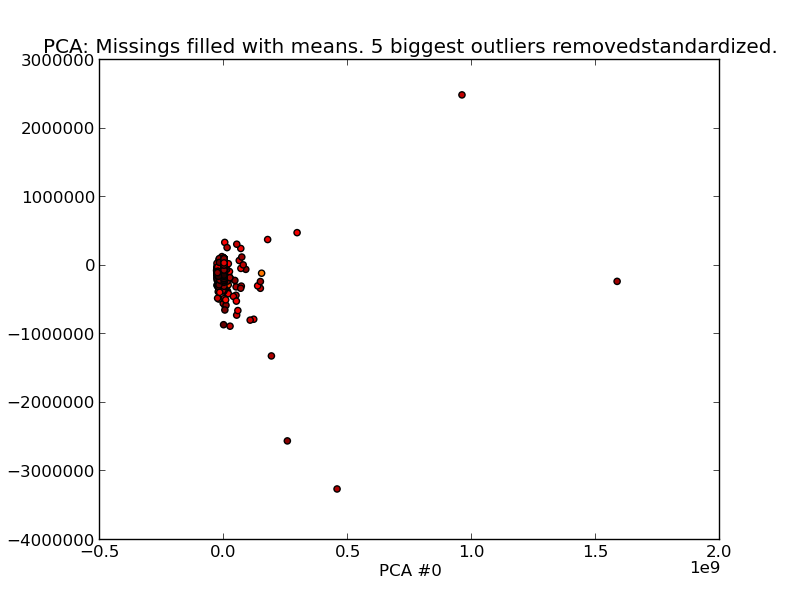
\includegraphics[width=0.9\textwidth]{pca/missings-filled-w-means_5-biggest-outliers-removed_standrd_}
\label{fig:prenorm_attrrem_0out}
\caption{PCA, where missing values have been replaced with means. Also the 5 biggest outliers from before have been removed prior to PCA.}
\end{figure}

Investigating the work others have performed on the data, leads us to believe that considerably better preprocessing can be done to the data. As an example, we have performed principal component analysis also on the normalized data set produced by [WHO].

\begin{figure}[H]
\centering
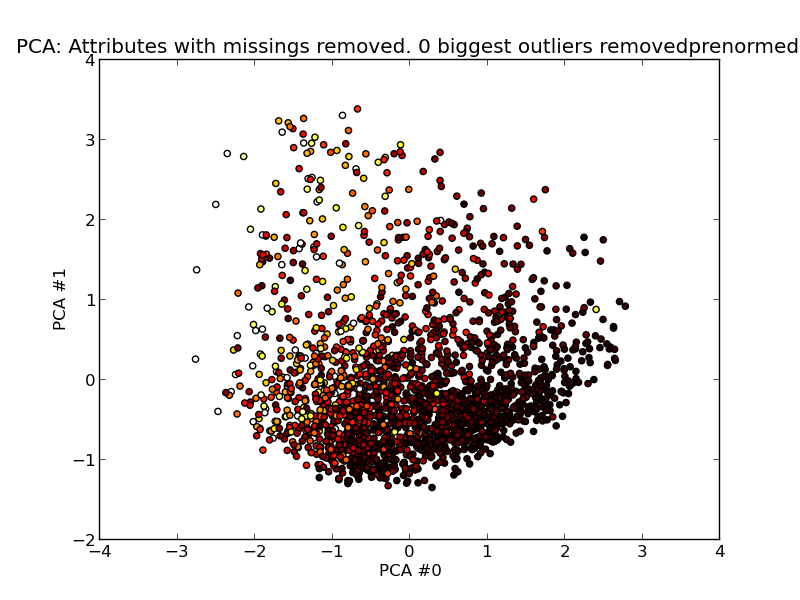
\includegraphics[width=0.9\textwidth]{pca/attr-with-missings-removed_0-biggest-outliers-removed_prenormed_}
\label{fig:prenorm_attrrem_0out}
\caption{Using normalized data from other source, attributes with missing values are removed.}
\end{figure}

The above data also appears to be normally distributed, in contrast to our own PCA. The first principal component also seems to capture quite well the amount of auto theft.

\begin{figure}[H]
\centering
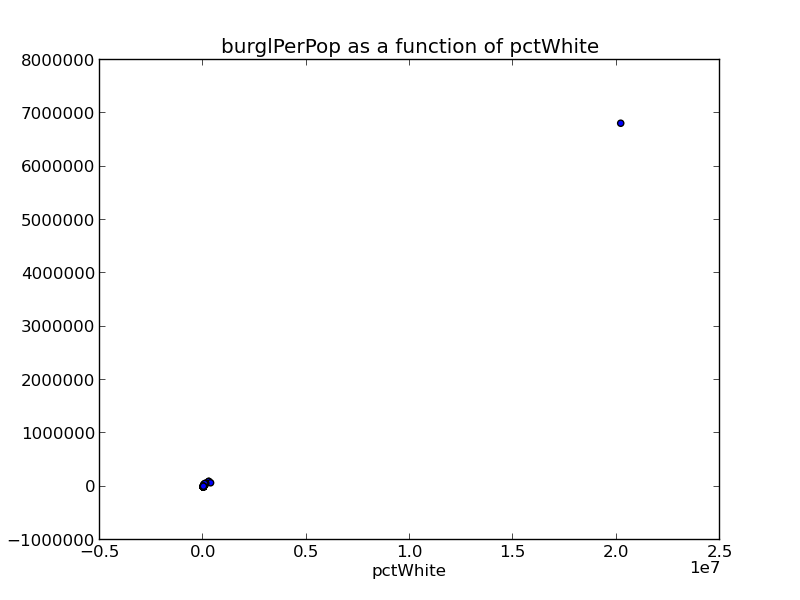
\includegraphics[width=0.9\textwidth]{correlations/burglPerPop-as-func-of-pctWhite.png}
\label{fig:prenorm_attrrem_0out}
\caption{Burgleries per population (1K people) as function of percentage of white population.}
\end{figure}

Many of our attributes have little correlation, as seen above, which is why regression is an obvious machine learning task. Looking at the normalized data by [WHO], furthermore leads us to believe that the task is feasable.

There are, however, some obvious attributes with high correlation, like population and auto theft, as seen below.

\begin{figure}[H]
\centering
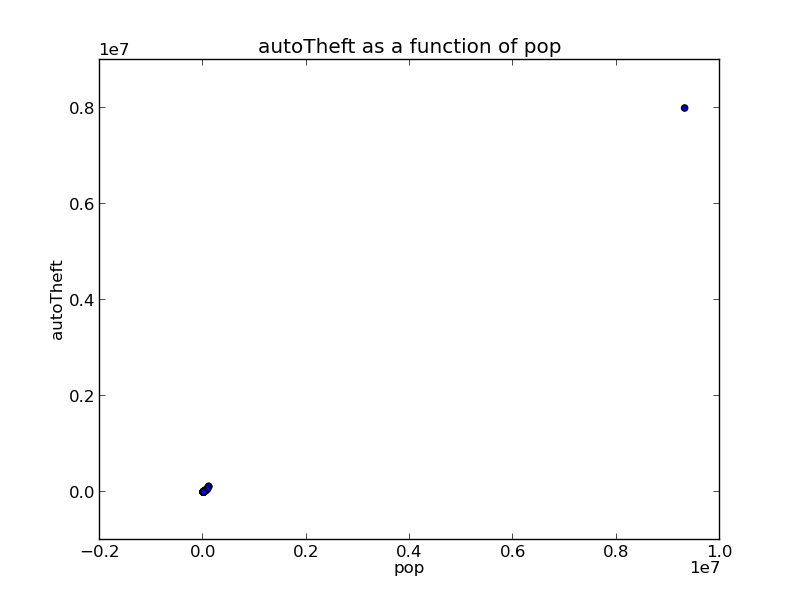
\includegraphics[width=0.9\textwidth]{correlations/autoTheft-as-func-of-pop}
\label{fig:prenorm_attrrem_0out}
\caption{Auto theft as function of population.}
\end{figure}

We realize now, that a possible problem with our principal component analysis is that we kept all of the violent crime attributes, which have very high correlation.

\section{Conclusion}
From looking at the normalized data from others' work, we have learned that better or additional preprocessing should be possible. We've also learned that almost all of our attributes are of the continuous ratio type. Based on our analysis (and the success of other similar analyses by others), we think that performing regression on the data to predict auto theft should be very much possible.

\section{Appendix}

\begin{figure}
\centering
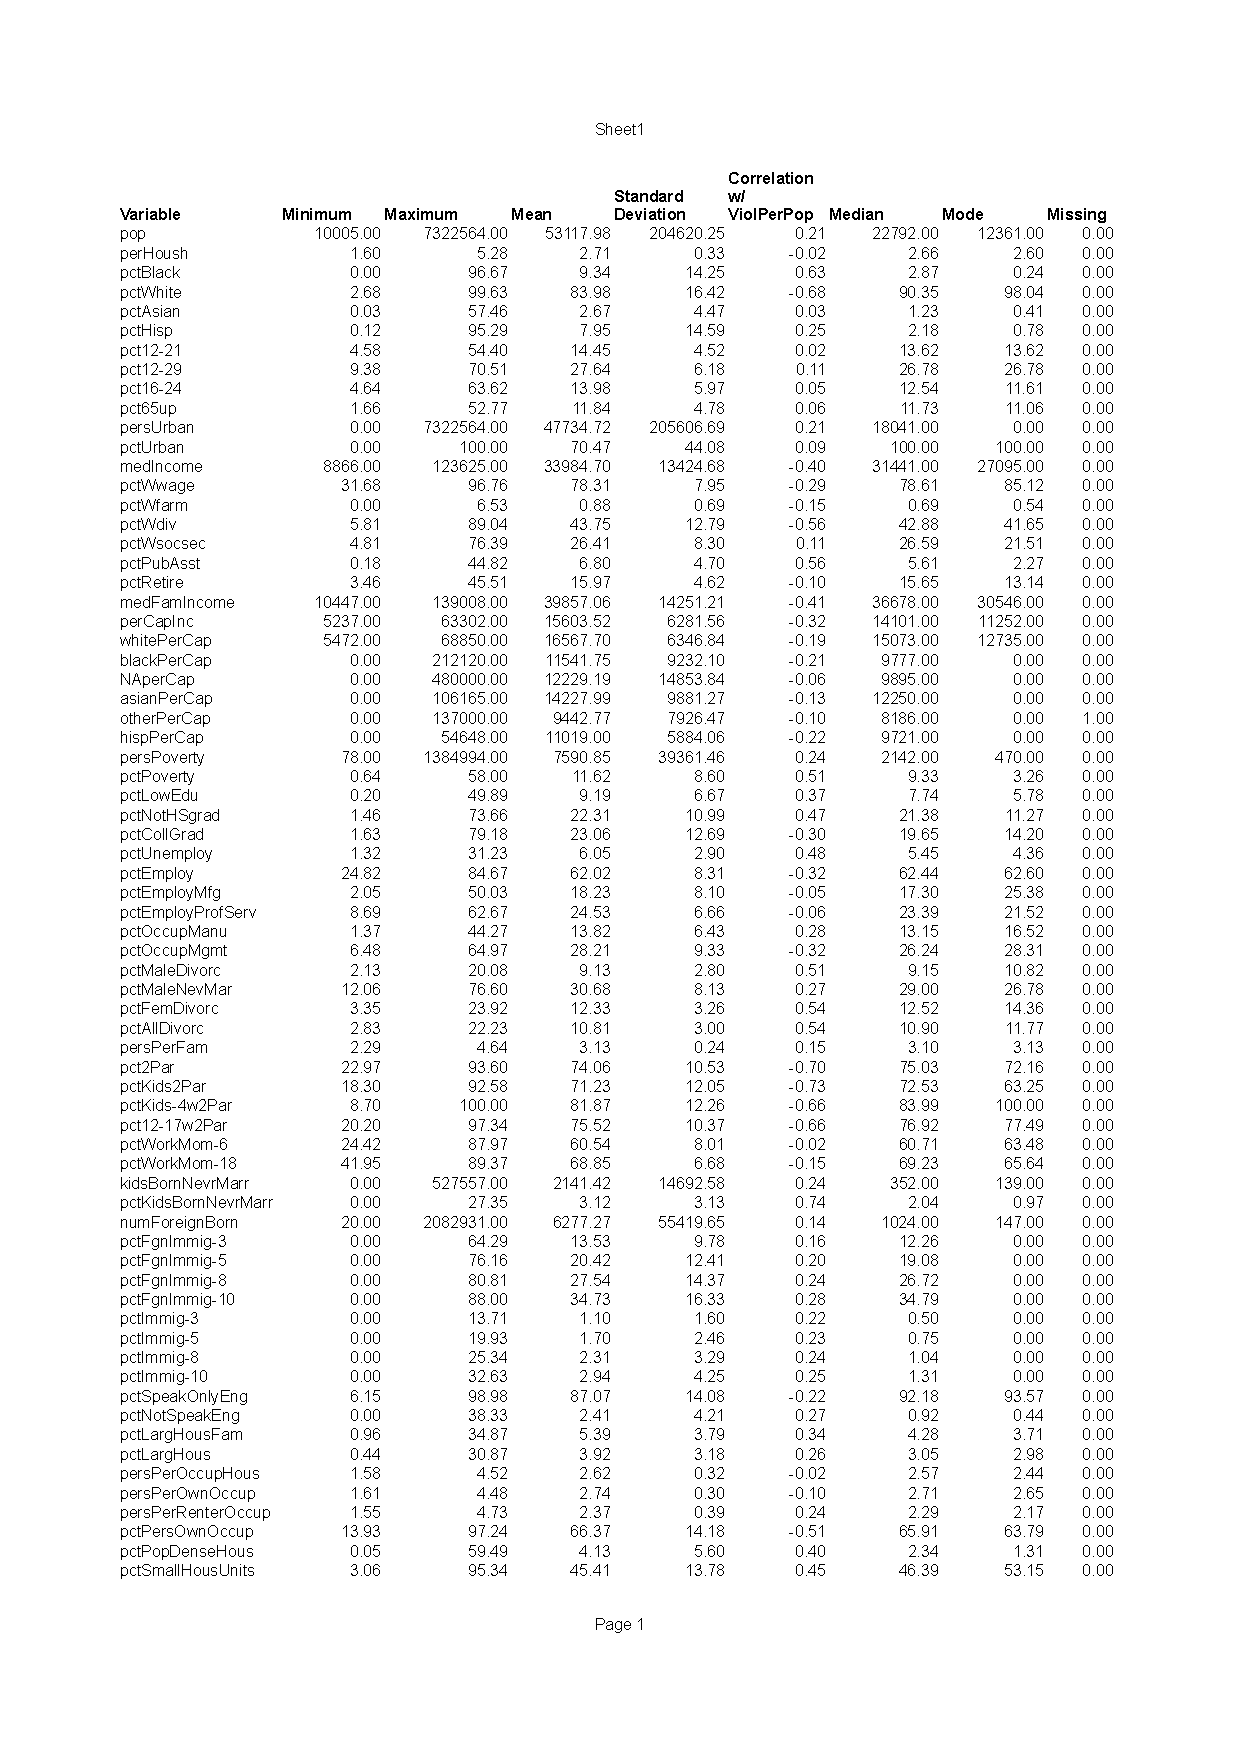
\includegraphics[h, width=1.3\textwidth]{sumstat1.pdf}
\end{figure}
\begin{figure}
\centering
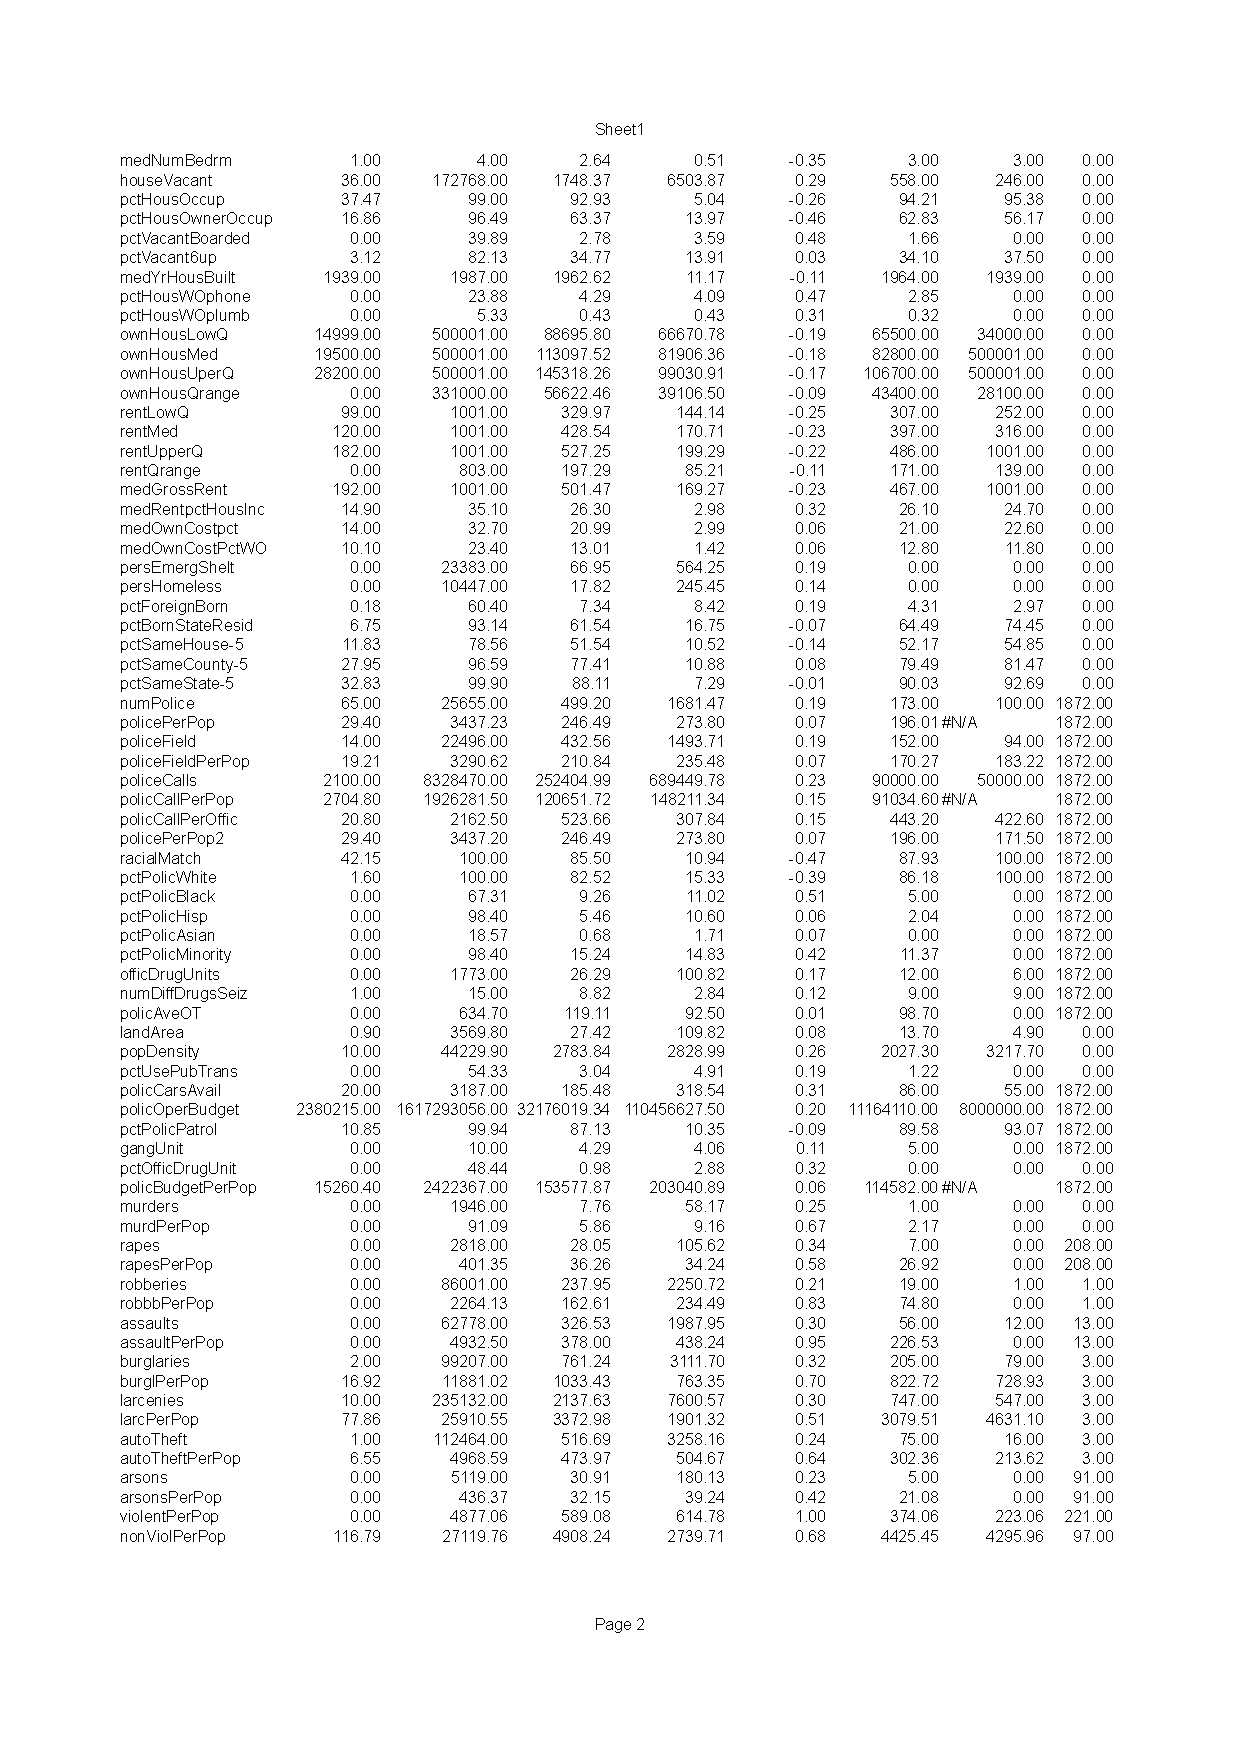
\includegraphics[h, width=1.3\textwidth]{sumstat2.pdf}
\end{figure}



% Bibliography
\newpage
\bibliographystyle{plain}
\bibliography{bachelorprojekt}
\end{document}
